% Created by tikzDevice version 0.8.1 on 2017-03-27 20:06:38
% !TEX encoding = UTF-8 Unicode
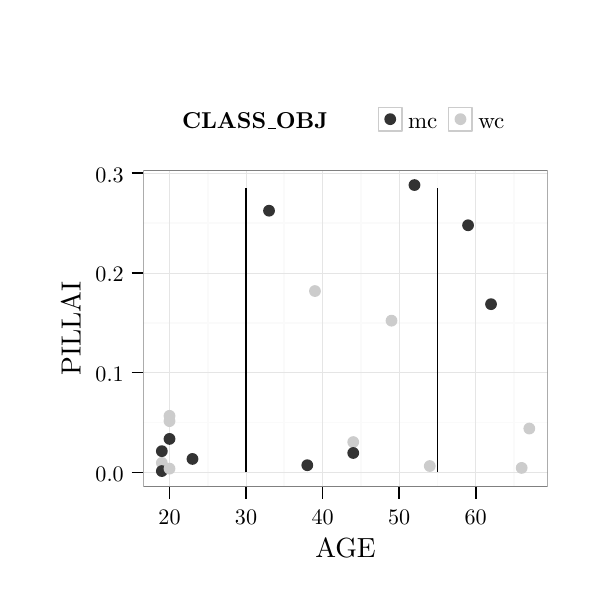
\begin{tikzpicture}[x=1pt,y=1pt]
\definecolor{fillColor}{RGB}{255,255,255}
\path[use as bounding box,fill=fillColor,fill opacity=0.00] (0,0) rectangle (202.36,202.36);
\begin{scope}
\path[clip] (  0.00,  0.00) rectangle (202.36,202.36);
\definecolor{drawColor}{RGB}{255,255,255}
\definecolor{fillColor}{RGB}{255,255,255}

\path[draw=drawColor,line width= 0.6pt,line join=round,line cap=round,fill=fillColor] ( -0.00,  0.00) rectangle (202.36,202.36);
\end{scope}
\begin{scope}
\path[clip] ( 41.84, 36.45) rectangle (187.90,150.69);
\definecolor{fillColor}{RGB}{255,255,255}

\path[fill=fillColor] ( 41.84, 36.45) rectangle (187.90,150.69);
\definecolor{drawColor}{gray}{0.98}

\path[draw=drawColor,line width= 0.6pt,line join=round] ( 41.84, 59.67) --
	(187.90, 59.67);

\path[draw=drawColor,line width= 0.6pt,line join=round] ( 41.84, 95.74) --
	(187.90, 95.74);

\path[draw=drawColor,line width= 0.6pt,line join=round] ( 41.84,131.81) --
	(187.90,131.81);

\path[draw=drawColor,line width= 0.6pt,line join=round] ( 65.08, 36.45) --
	( 65.08,150.69);

\path[draw=drawColor,line width= 0.6pt,line join=round] ( 92.74, 36.45) --
	( 92.74,150.69);

\path[draw=drawColor,line width= 0.6pt,line join=round] (120.41, 36.45) --
	(120.41,150.69);

\path[draw=drawColor,line width= 0.6pt,line join=round] (148.07, 36.45) --
	(148.07,150.69);

\path[draw=drawColor,line width= 0.6pt,line join=round] (175.73, 36.45) --
	(175.73,150.69);
\definecolor{drawColor}{gray}{0.90}

\path[draw=drawColor,line width= 0.2pt,line join=round] ( 41.84, 41.64) --
	(187.90, 41.64);

\path[draw=drawColor,line width= 0.2pt,line join=round] ( 41.84, 77.71) --
	(187.90, 77.71);

\path[draw=drawColor,line width= 0.2pt,line join=round] ( 41.84,113.78) --
	(187.90,113.78);

\path[draw=drawColor,line width= 0.2pt,line join=round] ( 41.84,149.85) --
	(187.90,149.85);

\path[draw=drawColor,line width= 0.2pt,line join=round] ( 51.25, 36.45) --
	( 51.25,150.69);

\path[draw=drawColor,line width= 0.2pt,line join=round] ( 78.91, 36.45) --
	( 78.91,150.69);

\path[draw=drawColor,line width= 0.2pt,line join=round] (106.57, 36.45) --
	(106.57,150.69);

\path[draw=drawColor,line width= 0.2pt,line join=round] (134.24, 36.45) --
	(134.24,150.69);

\path[draw=drawColor,line width= 0.2pt,line join=round] (161.90, 36.45) --
	(161.90,150.69);
\definecolor{fillColor}{gray}{0.20}

\path[fill=fillColor] (139.77,145.49) circle (  2.13);
\definecolor{fillColor}{gray}{0.80}

\path[fill=fillColor] ( 51.25, 62.10) circle (  2.13);
\definecolor{fillColor}{gray}{0.20}

\path[fill=fillColor] ( 87.21,136.22) circle (  2.13);
\definecolor{fillColor}{gray}{0.80}

\path[fill=fillColor] ( 48.48, 45.08) circle (  2.13);

\path[fill=fillColor] (178.50, 43.28) circle (  2.13);
\definecolor{fillColor}{gray}{0.20}

\path[fill=fillColor] ( 51.25, 53.75) circle (  2.13);

\path[fill=fillColor] ( 59.55, 46.52) circle (  2.13);

\path[fill=fillColor] (167.43,102.45) circle (  2.13);
\definecolor{fillColor}{gray}{0.80}

\path[fill=fillColor] (103.81,107.19) circle (  2.13);

\path[fill=fillColor] (117.64, 52.62) circle (  2.13);

\path[fill=fillColor] (131.47, 96.48) circle (  2.13);

\path[fill=fillColor] (181.26, 57.51) circle (  2.13);

\path[fill=fillColor] (145.30, 43.96) circle (  2.13);
\definecolor{fillColor}{gray}{0.20}

\path[fill=fillColor] ( 48.48, 49.33) circle (  2.13);

\path[fill=fillColor] (159.13,130.96) circle (  2.13);

\path[fill=fillColor] (117.64, 48.68) circle (  2.13);

\path[fill=fillColor] ( 48.48, 42.14) circle (  2.13);

\path[fill=fillColor] (101.04, 44.25) circle (  2.13);
\definecolor{fillColor}{gray}{0.80}

\path[fill=fillColor] ( 51.25, 60.19) circle (  2.13);

\path[fill=fillColor] ( 51.25, 43.02) circle (  2.13);
\definecolor{drawColor}{RGB}{0,0,0}

\path[draw=drawColor,line width= 0.6pt,line join=round] ( 78.91, 41.64) -- ( 78.91,144.44);

\path[draw=drawColor,line width= 0.6pt,line join=round] (148.07, 41.64) -- (148.07,144.44);
\definecolor{drawColor}{gray}{0.50}

\path[draw=drawColor,line width= 0.6pt,line join=round,line cap=round] ( 41.84, 36.45) rectangle (187.90,150.69);
\end{scope}
\begin{scope}
\path[clip] (  0.00,  0.00) rectangle (202.36,202.36);
\definecolor{drawColor}{RGB}{0,0,0}

\node[text=drawColor,anchor=base east,inner sep=0pt, outer sep=0pt, scale=  0.80] at ( 34.73, 38.33) {0.0};

\node[text=drawColor,anchor=base east,inner sep=0pt, outer sep=0pt, scale=  0.80] at ( 34.73, 74.40) {0.1};

\node[text=drawColor,anchor=base east,inner sep=0pt, outer sep=0pt, scale=  0.80] at ( 34.73,110.47) {0.2};

\node[text=drawColor,anchor=base east,inner sep=0pt, outer sep=0pt, scale=  0.80] at ( 34.73,146.54) {0.3};
\end{scope}
\begin{scope}
\path[clip] (  0.00,  0.00) rectangle (202.36,202.36);
\definecolor{drawColor}{RGB}{0,0,0}

\path[draw=drawColor,line width= 0.6pt,line join=round] ( 37.58, 41.64) --
	( 41.84, 41.64);

\path[draw=drawColor,line width= 0.6pt,line join=round] ( 37.58, 77.71) --
	( 41.84, 77.71);

\path[draw=drawColor,line width= 0.6pt,line join=round] ( 37.58,113.78) --
	( 41.84,113.78);

\path[draw=drawColor,line width= 0.6pt,line join=round] ( 37.58,149.85) --
	( 41.84,149.85);
\end{scope}
\begin{scope}
\path[clip] (  0.00,  0.00) rectangle (202.36,202.36);
\definecolor{drawColor}{RGB}{0,0,0}

\path[draw=drawColor,line width= 0.6pt,line join=round] ( 51.25, 32.18) --
	( 51.25, 36.45);

\path[draw=drawColor,line width= 0.6pt,line join=round] ( 78.91, 32.18) --
	( 78.91, 36.45);

\path[draw=drawColor,line width= 0.6pt,line join=round] (106.57, 32.18) --
	(106.57, 36.45);

\path[draw=drawColor,line width= 0.6pt,line join=round] (134.24, 32.18) --
	(134.24, 36.45);

\path[draw=drawColor,line width= 0.6pt,line join=round] (161.90, 32.18) --
	(161.90, 36.45);
\end{scope}
\begin{scope}
\path[clip] (  0.00,  0.00) rectangle (202.36,202.36);
\definecolor{drawColor}{RGB}{0,0,0}

\node[text=drawColor,anchor=base,inner sep=0pt, outer sep=0pt, scale=  0.80] at ( 51.25, 22.72) {20};

\node[text=drawColor,anchor=base,inner sep=0pt, outer sep=0pt, scale=  0.80] at ( 78.91, 22.72) {30};

\node[text=drawColor,anchor=base,inner sep=0pt, outer sep=0pt, scale=  0.80] at (106.57, 22.72) {40};

\node[text=drawColor,anchor=base,inner sep=0pt, outer sep=0pt, scale=  0.80] at (134.24, 22.72) {50};

\node[text=drawColor,anchor=base,inner sep=0pt, outer sep=0pt, scale=  0.80] at (161.90, 22.72) {60};
\end{scope}
\begin{scope}
\path[clip] (  0.00,  0.00) rectangle (202.36,202.36);
\definecolor{drawColor}{RGB}{0,0,0}

\node[text=drawColor,anchor=base,inner sep=0pt, outer sep=0pt, scale=  1.00] at (114.87, 10.84) {AGE};
\end{scope}
\begin{scope}
\path[clip] (  0.00,  0.00) rectangle (202.36,202.36);
\definecolor{drawColor}{RGB}{0,0,0}

\node[text=drawColor,rotate= 90.00,anchor=base,inner sep=0pt, outer sep=0pt, scale=  1.00] at ( 19.11, 93.57) {PILLAI};
\end{scope}
\begin{scope}
\path[clip] (  0.00,  0.00) rectangle (202.36,202.36);
\definecolor{fillColor}{RGB}{255,255,255}

\path[fill=fillColor] ( 51.50,160.76) rectangle (178.24,177.83);
\end{scope}
\begin{scope}
\path[clip] (  0.00,  0.00) rectangle (202.36,202.36);
\definecolor{drawColor}{RGB}{0,0,0}

\node[text=drawColor,anchor=base west,inner sep=0pt, outer sep=0pt, scale=  0.83] at ( 55.77,165.88) {\bfseries CLASS{\_{}}OBJ};
\end{scope}
\begin{scope}
\path[clip] (  0.00,  0.00) rectangle (202.36,202.36);
\definecolor{drawColor}{gray}{0.80}
\definecolor{fillColor}{RGB}{255,255,255}

\path[draw=drawColor,line width= 0.6pt,line join=round,line cap=round,fill=fillColor] (126.74,165.03) rectangle (135.27,173.56);
\end{scope}
\begin{scope}
\path[clip] (  0.00,  0.00) rectangle (202.36,202.36);
\definecolor{fillColor}{gray}{0.20}

\path[fill=fillColor] (131.01,169.29) circle (  2.13);
\end{scope}
\begin{scope}
\path[clip] (  0.00,  0.00) rectangle (202.36,202.36);
\definecolor{drawColor}{gray}{0.80}
\definecolor{fillColor}{RGB}{255,255,255}

\path[draw=drawColor,line width= 0.6pt,line join=round,line cap=round,fill=fillColor] (152.12,165.03) rectangle (160.66,173.56);
\end{scope}
\begin{scope}
\path[clip] (  0.00,  0.00) rectangle (202.36,202.36);
\definecolor{fillColor}{gray}{0.80}

\path[fill=fillColor] (156.39,169.29) circle (  2.13);
\end{scope}
\begin{scope}
\path[clip] (  0.00,  0.00) rectangle (202.36,202.36);
\definecolor{drawColor}{RGB}{0,0,0}

\node[text=drawColor,anchor=base west,inner sep=0pt, outer sep=0pt, scale=  0.83] at (137.44,165.85) {mc};
\end{scope}
\begin{scope}
\path[clip] (  0.00,  0.00) rectangle (202.36,202.36);
\definecolor{drawColor}{RGB}{0,0,0}

\node[text=drawColor,anchor=base west,inner sep=0pt, outer sep=0pt, scale=  0.83] at (162.82,165.85) {wc};
\end{scope}
\end{tikzpicture}
